\chapter{Конструкторская часть}

В данной главе представлены требования к разрабатываемому программному обеспечению, приведены схемы алгоритмов и введена модель вычислений для проведения теоретической оценки трудоёмкости.

\section{Требования к программе}

Для разрабатываемой программы определены следующие задачи:
\begin{enumerate}
	\item реализовать интерфейс выбора операций для пользователя;
	\item обеспечить возможность работы программы в двух режимах: одиночное выполнение и массовое измерение времени выполнения;
	\item в режиме одиночного запуска предусмотреть:
	\begin{itemize}
		\item ввод размеров и элементов двух матриц;
		\item проверку корректности введённых данных;
		\item проверку совместимости матриц для операции умножения;
	\end{itemize}
	\item в режиме массового измерения времени фиксировать затраченное процессорное время и выводить результаты в табличном виде.
\end{enumerate}

\section{Разработка алгоритмов}

На рисунке~\ref{pic_simple_scheme} представлена схема стандартного алгоритма перемножения матриц. Рисунки~\ref{pic_vinograd_1}--\ref{pic_vinograd_2} демонстрируют структуру алгоритма Винограда.

\begin{figure}[h!]
	\center{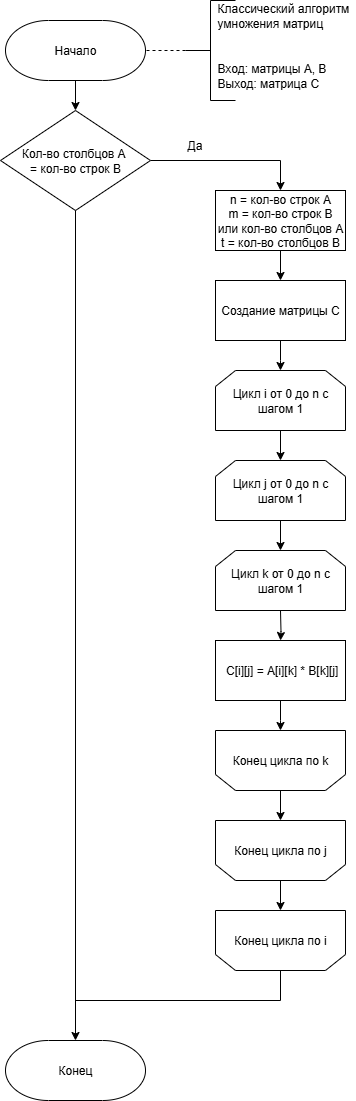
\includegraphics[height=24.7cm]{images/simple_scheme}}
	\caption{Схема стандартного алгоритма умножения матриц}
	\label{pic_simple_scheme}
\end{figure}
\clearpage

\begin{figure}[h!]
	\center{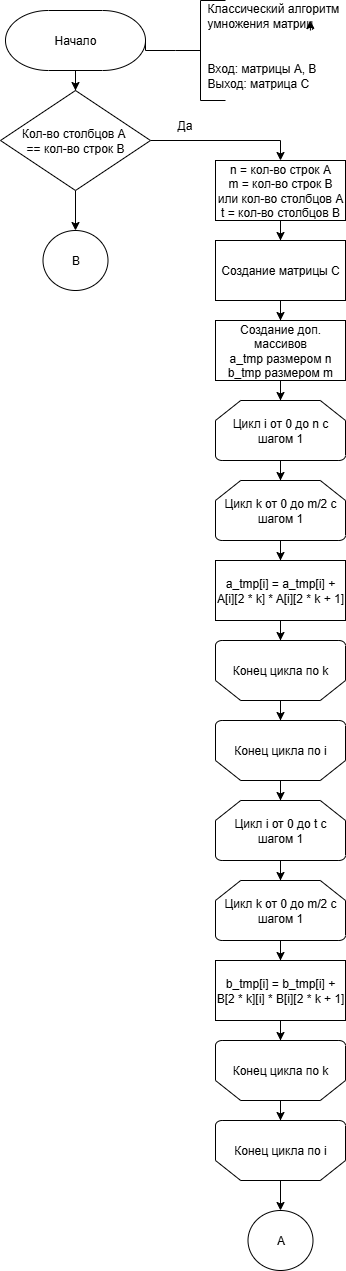
\includegraphics[height=24.7cm]{images/vinograd_scheme_1}}
	\caption{Схема алгоритма Винограда (часть 1)}
	\label{pic_vinograd_1}
\end{figure}
\clearpage

\begin{figure}[h!]
	\center{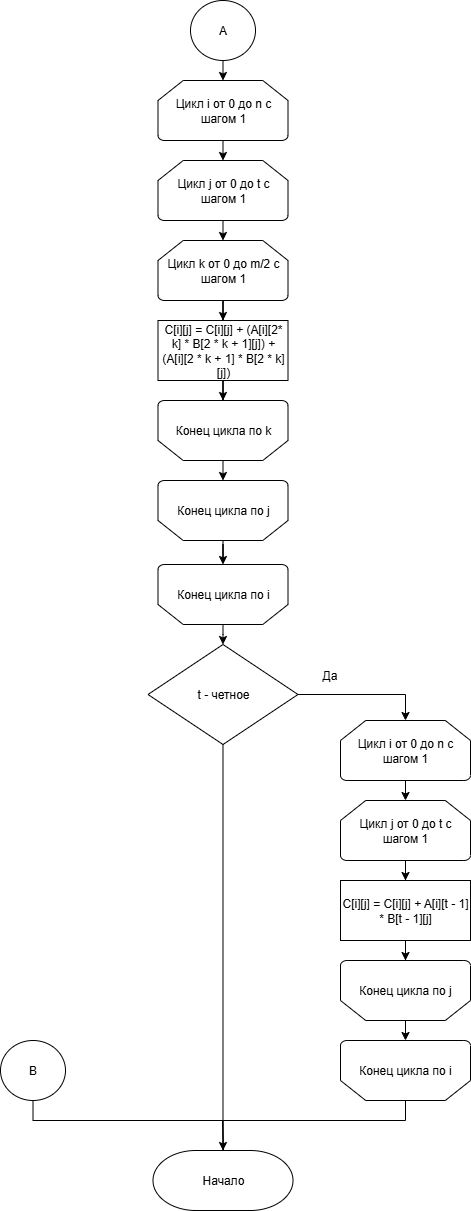
\includegraphics[height=24.7cm]{images/vinograd_scheme_2}}
	\caption{Схема алгоритма Винограда (часть 2)}
	\label{pic_vinograd_2}
\end{figure}
\clearpage

Для алгоритма Винограда были предложены следующие пути оптимизации:
\begin{enumerate}
	\item использование предварительно вычисленных значений (например, $N-1$, $N/2$);
	\item хранение промежуточных сумм в буферах при заполнении массивов и результирующей матрицы.
\end{enumerate}

На рисунках~\ref{pic_vinograd_opt_scheme_1}--\ref{pic_vinograd_opt_scheme_2} представлена схема оптимизированного алгоритма Винограда.

\begin{figure}[h!]
	\center{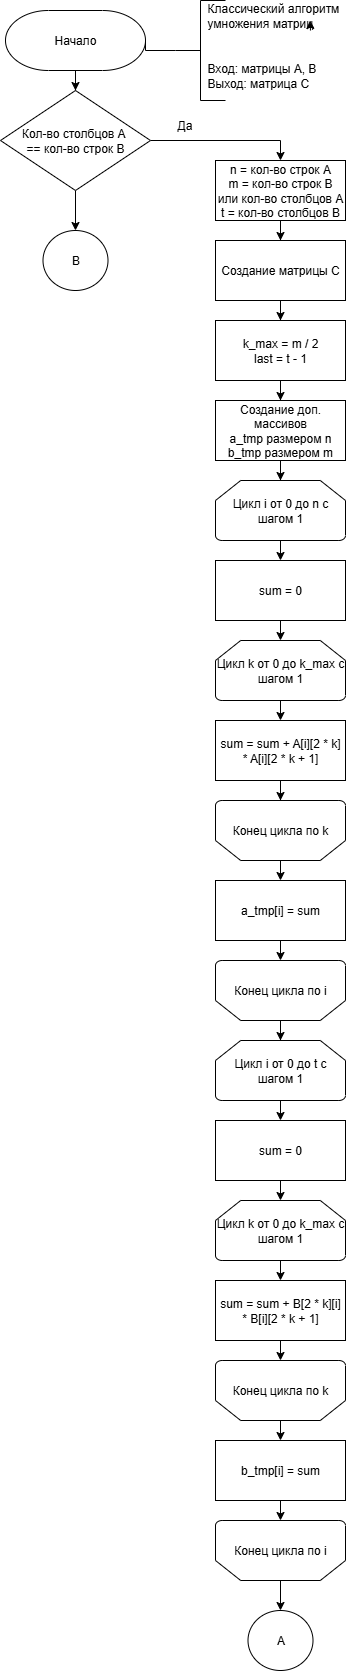
\includegraphics[height=24.7cm]{images/vinograd_opt_scheme_1}}
	\caption{Схема оптимизированного алгоритма Винограда (часть 1)}
	\label{pic_vinograd_opt_scheme_1}
\end{figure}
\clearpage

\begin{figure}[h!]
	\center{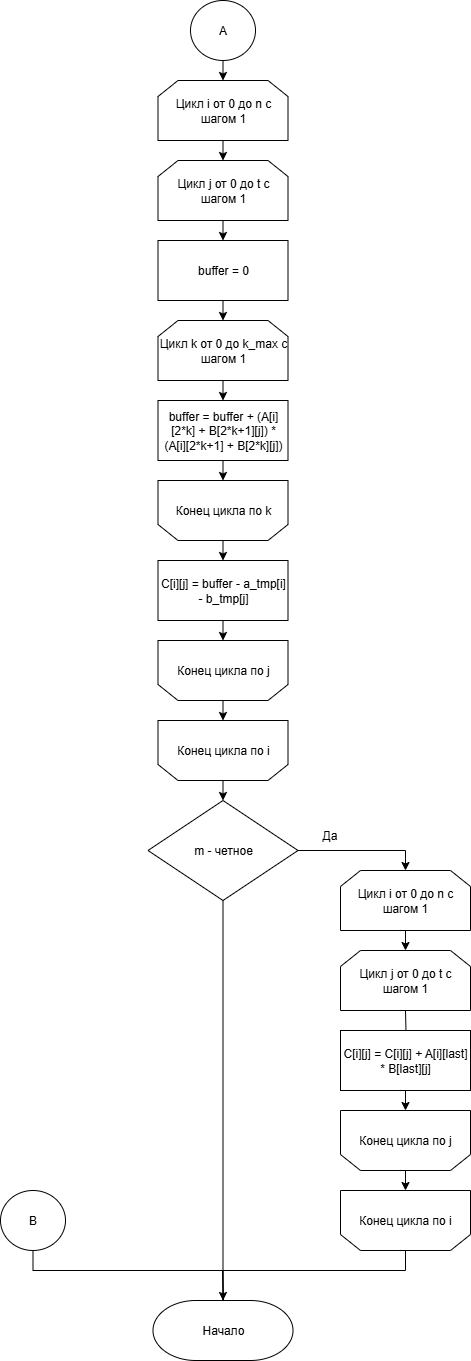
\includegraphics[height=24.7cm]{images/vinograd_opt_scheme_2}}
	\caption{Схема оптимизированного алгоритма Винограда (часть 2)}
	\label{pic_vinograd_opt_scheme_2}
\end{figure}
\clearpage

\section{Модель вычислений}

Для анализа трудоёмкости алгоритмов вводится следующая модель:
\begin{enumerate}
	\item стоимость операций $=, ==, !=, >, <, >=, <=, \&\&, ||, \&=, |=,$ $+=,$ $-=,$ $+,$ $-,$ $[],$ $ ++,$ $--,$ $<<,$ $>>$ принимается равной 1;
	\item стоимость операций $\cdot, /, \cdot=, /=, \%, \%=$ принимается равной 2;
	\item трудоёмкость условного оператора вида \textit{if (Условие) \{Блок X\} else \{Блок Y\}}, где вычисление условия и блоков X и Y обозначено как $c_{cond}$, $c_x$, $c_y$, оценивается по формуле~(\ref{if_complexity}):
	\begin{equation}
		\label{if_complexity}
		c_{if} = c_{cond} + 
		\begin{cases}
			\min(c_x, c_y), & \text{лучший случай} \\
			\max(c_x, c_y), & \text{худший случай}
		\end{cases}
	\end{equation}
	\item трудоёмкость цикла вида \textit{for (Начало, Условие, Приращение) \{тело\}}, где трудоёмкость начальной установки, условия, приращения и тела соответственно равны $c_{start}, c_{cond}, c_{step}, c_{body}$, вычисляется по формуле~(\ref{for_complexity}), где $M$ --- число итераций:
	\begin{equation}
		\label{for_complexity}
		c_{for} = c_{start} + c_{cond} + M \cdot (c_{body} + c_{step} + c_{cond})
	\end{equation}
\end{enumerate}

\section{Расчёт трудоёмкости алгоритмов}

\subsection{Стандартный алгоритм}

Трудоёмкость стандартного алгоритма (рисунок~\ref{pic_simple_scheme}) складывается из трёх вложенных циклов и набора операций во внутреннем цикле. Итоговая трудоёмкость рассчитывается по формуле~(\ref{eq_classic}):
\begin{equation}
	\label{eq_classic}
	f_{std} = 2 + P \cdot (2 + 2 + Q \cdot (2 + 2 + R \cdot (2 + 12))) = 14 P Q R + 4 P Q + 4 P + 2 \approx 14 P Q R
\end{equation}
где $P$, $Q$, $R$ — размеры соответствующих измерений исходных матриц.

\subsection{Алгоритм Винограда}

Алгоритм Винограда состоит из четырёх этапов:

\begin{enumerate}
	\item \textbf{заполнение массива \textit{mulH}}:  
	Для каждой строки A суммируются произведения пар элементов.  
	\begin{equation}
		f_1 = 2 + M \cdot (2 + 1 + 4 + \frac{N}{2} \cdot (4 + 1 + 6 + 2 + 3 \cdot 2)) = \frac{19}{2} MN + 7M + 2 \approx \frac{19}{2} MN
	\end{equation}
	
	\item \textbf{заполнение массива \textit{mulV}}:  
	Для каждого столбца B вычисляются промежуточные суммы.  
	\begin{equation}
		f_2 = 2 + K \cdot (2 + 1 + 4 + \frac{N}{2} \cdot (4 + 1 + 6 + 2 + 3 \cdot 2)) = \frac{19}{2} KN + 7K + 2 \approx \frac{19}{2} KN
	\end{equation}
	
	\item \textbf{заполнение матрицы \textit{C}}:  
	Используются заранее посчитанные суммы. Каждое вычисление ячейки включает доступы к буферам, сложения, умножения и корректировку.  
	\begin{equation}
		f_3 = 2 + M \cdot (2 + 2 + K \cdot (2 + 4 + 1 + 2 + 4 + \frac{N}{2} \cdot (4 + 12 + 1 + 5 + 5 \cdot 2))) = 16 M N K + 13 M K + 4 M + 2 \approx 16 M N K
	\end{equation}
	
	\item \textbf{корректировка для нечётного N}:  
	\begin{equation}
		f_{if} = 
		\begin{cases}
			3, & N \text{ — чётное} \\
			16 M K + 4 M + 5, & N \text{ — нечётное}
		\end{cases}
	\end{equation}
\end{enumerate}

Общая трудоёмкость:

\begin{equation}
	f_{total} = 
	\begin{cases}
		16 M N K + 13 M K + \frac{19}{2}(MN + KN) + 11 M + 7 K + 9, & N \text{ — чётное} \\
		16 M N K + 29 M K + \frac{19}{2}(MN + KN) + 15 M + 7 K + 11, & N \text{ — нечётное}
	\end{cases}
\end{equation}

\subsection{Оптимизированный алгоритм Винограда}

В оптимизированном алгоритме Винограда введены улучшения: предварительное вычисление промежуточных значений ($N-1$, $N/2$ и др.) и использование буферов для накопления промежуточных сумм при заполнении массивов и результирующей матрицы. Эти меры сокращают количество арифметических операций и обращений к памяти.

Трудоёмкость этапов алгоритма (см. рисунки~\ref{pic_vinograd_opt_scheme_1}--\ref{pic_vinograd_opt_scheme_2}) оценивается следующим образом:

\begin{enumerate}
	\item \textbf{заполнение массива \textit{mulH}.}  
	Сумма произведений элементов строк первой матрицы вычисляется заранее и сохраняется в буфер \textit{tmp\_a}. Трудоёмкость этого этапа задаётся формулой:
	\begin{equation}
		f_1 = 2 + P \cdot \left(2 + 1 + 2 + \frac{Q}{2} \cdot (2 + 1 + 6 + 1 + 1 + 1 \cdot 2) \right) 
		= \frac{13}{2} P Q + 5 P + 2 \approx \frac{13}{2} P Q
	\end{equation}
	
	\item \textbf{заполнение массива \textit{mulV}.}  
	Аналогично формируется буфер \textit{tmp\_b} для столбцов второй матрицы:
	\begin{equation}
		f_2 = 2 + R \cdot \left(2 + 1 + 2 + \frac{Q}{2} \cdot (2 + 1 + 6 + 1 + 1 + 1 \cdot 2) \right)
		= \frac{13}{2} R Q + 5 R + 2 \approx \frac{13}{2} R Q
	\end{equation}
	
	\item \textbf{вычисление результирующей матрицы \textit{C}.}  
	Основные вычисления включают использование предварительно накопленных сумм из буферов и коррекцию для нечётного $Q$:
	
	\begin{enumerate}
		\item для чётного $Q$:
		\begin{multline}
			f_{31} = 3 + 2 + M \cdot \Bigl(2 + 2 + K \cdot (2 + 4 + 1 + 2 + 2 + \frac{Q}{2} \cdot \\
			(2 + 12 + 1 + 3 + 2 + 1 \cdot 2)) \Bigr) 
			= 11 P Q R + 11 P R + 4 P + 5 \approx 11 P Q R
		\end{multline}
		
		\item для нечётного $Q$:
		\begin{multline}
			f_{32} = 3 + 2 + M \cdot \Bigl(2 + 2 + K \cdot (2 + 8 + 1 + 4 + 1 + 1 \cdot 2 + \frac{Q}{2} \cdot \\
			(2 + 12 + 1 + 3 + 2 + 1 \cdot 2)) \Bigr) 
			= 11 P Q R + 18 P R + 4 P + 5 \approx 11 P Q R
		\end{multline}
	\end{enumerate}
\end{enumerate}

Таким образом, суммарная трудоёмкость оптимизированного алгоритма Винограда вычисляется по формуле:
\begin{equation}
	f_{total} = 
	\begin{cases}
		11 P Q R + 11 P R + \frac{13}{2} (P Q + R Q) + 9 P + 5 R + 7, & \text{л.с. ($Q$ --- чётное)} \\
		11 P Q R + 18 P R + \frac{13}{2} (P Q + R Q) + 9 P + 5 R + 7, & \text{х.с. ($Q$ --- нечётное)}
	\end{cases}
\end{equation}

\textbf{Вывод.}  
Предварительное вычисление промежуточных сумм и использование буферов позволяют сократить число операций. Оптимизированный алгоритм Винограда улучшает трудоёмкость примерно в 1.27 раза по сравнению с классическим алгоритмом и в 1.45 раза по сравнению с исходной версией алгоритма Винограда.
\clearpage